\begin{figure}
  \centering
  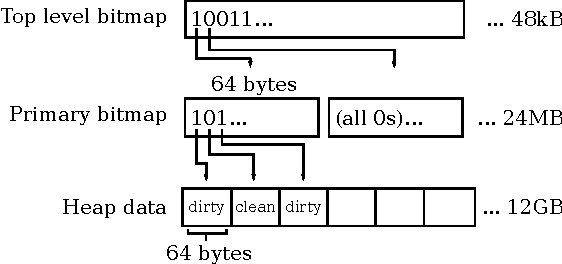
\includegraphics[width=.7\linewidth]{OLTP_design/bitset.pdf}
  \caption{\textbf{Hierarchical bitmap set.} Each bit of top level bitmap corresponds to a cache line of bits (64 bytes, 512 bits) in the primary bitmap; top level bit is set if any associated bits in primary bitmap are set (boolean \emph{or} operation).  Each bit in the primary bitmap corresponds to a cache line in the database buffer cache and is set if the cache line is dirty (contains modifications since the start of the batch).}
  \label{fig::bitset}
\end{figure}
